\section{Lack of features in the model}
\label{sec:lack}
When we startet to implement the model and simulate our two cases, we encountered some
problems that we did not foresee when we read the article \cite{self-org}, and the other
articles \cite{helbing00}, \cite{social-force}.
We encountered some special cases where the model did not suffice to give a realistic
simulation, and also we could not, from the articles, figure out how to fix some initial parameters.
In the articles the authors did not write of any such problems and how to deal with them,
so we had to come up with our own solutions to solve them, and thereby give a more realistic
simulation.
In the following section we discuss these problems and our solutions to these problems.

\subsection{Discussion on walls in special cases.}\label{wallEndpoints}
The wall is created as a vector. The repulsive force vector is perpendicular to the wall 
vector and has a direction directly towards the pedestrian $\alpha$.

In the general case of the repulsive force on a pedestrian, $\alpha$, from a wall 
nearby is given as a function of the vector from the nearest point. This point we 
calculate by finding the point that makes the vector form $\alpha$ to the wall be 
perpendicular to to vector that is the wall. In some cases though the point will not 
be on the wall it self. This of course makes no sense since you would then be 
repulsed by a non existing part of the wall meaning that you would avoid free 
areas. In this case you would have to use the end point of the wall. But doing this 
can make some unrealistic behaviour as well, if the walls have the right composition. 

Let's start out by looking at a case with no problem. A case with no problems is a 
room where the angles between the walls is less than $180^o$, i.e. a squared room 
where the angles are $90^o$. For a pedestrian close to the corner between two walls, you 
would calculate the repulsive force from both of the walls. This you do in order 
for the pedestrian to avoid going through either one of the walls. When you do 
this you get a force directly away from each of the walls. This clearly makes 
sense and there is no problem in doing so.

\subsubsection{Forces at kinks}
The case where the angle between two walls is greater than $180^o$ could on the 
other hand give some problems if not handled correctly. The case is sketched in 
figure \ref{fig:wallcase}. Here there are 3 different areas that a pedestrian $\alpha$ 
can be in. The area A where $\alpha$ is only perpendicular to wall $1$, in area B, 
$\alpha$ will not be perpendicular to any of the walls and in C he will be only 
perpendicular to wall 2. If a pedestrian is in area B then we would calculate the 
forces from the end point of the walls. This will be from the point where the two 
walls meet. This will give you a double repulsion from one point and that 
does not make sense. Also when you are in are A or C you would get a repulsive force 
from a second wall you would be of no risk of going into and in many situations 
could not see because the first wall is blocking the sight. This of course does not 
make any sense either. So the way that we handle this situation is the following. 
When the angle between the walls is greater than $180^o$, from pedestrian $\alpha$'s 
point of view, you should look at the two walls as one, and in that way you will 
only calculate one force from the walls. In area A or C only the closest point 
on the closest wall should affect you. In the case of $\alpha$ being in area B 
the walls themselves doesn't matter, only the vector going from the conjoint 
point of the walls to $\alpha$, should affect and only one time. Doing this, 
there should be no unrealistic scenarios concerning wall junctions and walls 
with more than $180^o$ between them. But this could create and undesired 
behaviour at doors of other objects created with free end points.

\begin{figure}[ht]
\centering
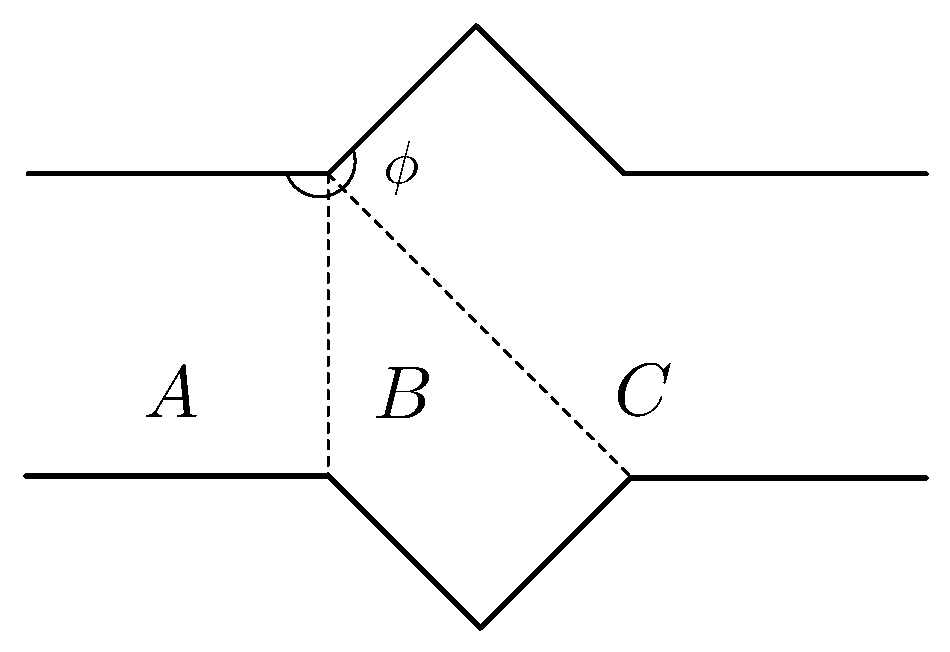
\includegraphics[scale=0.45]{Figures/WallCase.pdf} 
\caption{}\label{fig:wallcase}
\end{figure}

\subsubsection{The force at doorways}
We encountered a problem when dealing with doors. The problem arises because 
the door is constructed by two free endpoints and pedestrians feel a repulsion 
force from these points according to section \ref{wallEndpoints}. This means 
that a pedestrian trying to exit through the door will feel a repulsive force 
from both of the walls which prevent him from walking through the door. The second he 
passes through the door he will be pushed forward and accelerate which is unwanted 
behaviour. This we resolved by removing the force from free endpoint when:

\begin{equation}
\| y - w \| > R
\end{equation}

This creates what we could call a "non repulsion zone" see figure(Mikkel Lav Tegning!).
In rare cases it could happen that a pedestrian is trying to exit the room and he feels 
no repulsion because he is in the "non repulsive zone", he is then pushed sideways out 
of the "non repulsion zone" and suddenly he will feel a great repulsive force because 
he first "discovers" it when he is very close to the wall see figure(Mikkel Lav Tegning!).

\subsubsection{Calculating the repulsion from walls}
The calculation of repulsion from the walls is split in two parts for each 
actor: First all the points on the walls that will affect the actor is 
identified, then the repulsion from each point is calculated. As explained in 
section~\ref{sec:the-model}, the repulsion from the wall is measured from the 
nearest point of the wall to the actor. Identifying these points is done using 
the following algorithm:

\begin{enumerate}
    \item For each wall, calculate the projection of the vector pointing from 
        the wall's starting point to the actor, unto the vector pointing from 
        the wall's starting point to its endpoint.
        \begin{enumerate}
            \item If this point is part of the wall, save it to the list of points 
                repulsion should be calculated from, and add the wall's two endpoints 
                to the list of already used endpoints.

            \item If the projected point is not part of the wall, the endpoint closest 
                to the actor is used instead. This endpoint is saved to a 
                third list of endpoints repulsion should be calculated from.
        \end{enumerate}

    \item After having gone through all walls, for each point in the third 
        list, check if this point is already in the list of used endpoints. If 
        so, discard it. Otherwise, add it to the list of points repulsion 
        should be calculated from, and to the list of used endpoints.
\end{enumerate}

The algorithm starts out with the list of walls, and produces a list of points 
to calculate this repulsion from, ensuring that no wall endpoint is used 
twice. The points are then used as a basis for calculating the repulsion, as 
described in section~\ref{sec:the-model}.

\subsection{Initial conditions and constants}
When initialising the model, parameters are set for each pedestrian. In the 
model, every parameter can vary between actors, while in practice many of them 
do not. In this section, we go through the parameters and how they are set.  
For all random numbers, the operating system's built-in random number 
generator is used and considered to be sufficient for our purposes. We run 
multiple simulations of the same initial conditions by fixing the seed of the 
random number generator to the same value for each run. Distributions are 
drawn by using the distribution functions of the \emph{NumPy} mathematical 
library for Python \cite{numpy}.

\subsubsection{Position related parameters}
There are a number of parameters that are set that has to do with the initial 
position of actors and walls. Some where given, and some we had to come up
with ourselfs. They are:

\begin{itemize}
    \item \textbf{Wall endpoints:} Points describing the endpoints of the 
        walls. These are set according to the scenario we want to simulate, so 
        in a square room with a single exit in the middle of a wall, there 
        will be five wall segments (one on each side of the exit, and one for 
        each of the other walls).

    \item \textbf{Actor positions:} Each actor has a starting position 
        distributed randomly within the room. These are created by drawing a 
        set of random numbers for the x and y coordinates respectively, and 
        adjusting the range of this random number to be within the room's 
        dimensions. Actor positions are adjusted so that they do not overlap 
        with the walls by adjusting coordinates so that the distance from the 
        center to each wall is at most the radius. This adjustment is not made 
        between actors, so they may overlap initially. It is assumed that the 
        model will correct this within the first few simulation steps, which 
        is also what we have seen in practice.

    \item \textbf{Actor radii:} The actor radii are drawn from a normal 
        distribution with a mean of $0,2$ meters and a standard deviation of 
        $0,01$ meters. This is done to simulate a natural variety in physical 
        stature of humans, and to avoid deadlocks caused by perfectly 
        symmetrical forces that might otherwise occur \cite{helbing00}.
        %TODO: Check this reference, maybe better explanation?
\end{itemize}

\subsubsection{Movement related parameters}
A number of parameters are set to control the movement of the actors. They 
are:

\begin{itemize}
    \item \textbf{Target:} Each actor has a target that they move towards. 
        This target is set outside the exit actors will move towards, and is 
        the same for all actors when there is only one exit. In situations 
        where there are multiple exits, actors are set to move towards one of 
        the exits at random, regardless of their position within the room. 
        Since the model does not deal with pathfinding, targets are not 
        changed during the simulation. When an actor reaches its target, it is 
        considered to have escaped, and is removed from the simulation.

    \item \textbf{Initial velocity:} This is set as both a vector and a scalar 
        representing vector length. The scalar velocities are drawn from a 
        normal distribution with a mean of $1.34$ and a standard deviation of 
        $0,26$. The initial velocity vectors are created by multiplying the 
        scalar velocity with a normalised vector pointing from the actor's 
        initial position to the target.
        % TODO: Where do the mean and deviation come from?

    \item \textbf{Max speed:} TODO.

    \item \textbf{Desired velocity:} The desired velocity is the velocity the 
        actor wants to move at (see the explanation in 
        section~\ref{sec:the-model}). This is set equal to the initial velocity 
        under the assumption that when people start to leave a room they will 
        initially (try to) move at their desired velocity, and then be 
        affected by the model parameters once they start moving.

    \item \textbf{Relaxation time:} The relaxation time is the time it would 
        take an unhindered actor to return to their desired velocity after 
        having been hindered by something blocking their path. This is set to 
        one second for all actors.
        % TODO: Why one second, and is this explanation correct?

    \item \textbf{$\lambda$:} \cite{self-org} chose $\lambda$ $\approx 0.75$ to take into account
	anisotropic character of pedestrian interaction, such that the situations in front of
	a pedestrian have bigger impact on the pedestrians behavior than things going on
	behind them. By looking at eguation 44 we see that if we set $\lambda = 1$, the middle 
	paranthesis will be 1, and hence the personal sphere will only take into account the distance
	between agent $\alpha$ and $\beta$ and not their placement respect to each other. By setting $\lambda = 0$, the middle paranthesis will be
	$\frac{1+\cos{\phi}}{2}$
	and therefore the situation happending behind agent $\alpha$ would affect $\alpha$'s behavior.
	By setting $\lambda \approx 0.75$, the first part of eguation 44 is
	 $A_{\alpha}^{1} exp \left(
            \frac{ r_{\alpha \beta} - d_{\alpha \beta }}
                 {B_{\alpha}^1}
	    \right)
	  \vec{\eta_{\alpha \beta}} \cdot
	  \left(
	      0.75 + 0.25
		\frac{1+\cos{\phi}}{2}
	    \right)$,
	and  other agents behind $\alpha$ will only influence $\alpha$ with 25\% of what the influence would be without a $\lambda$.
	Even though the model is called a social force model, we will point out that it is not physical forces acting on agent $\alpha$ but
	rather motivation to act. This is more clear when adding $\lambda$, since Newton's 3'rd law (action = reaction) does not hold
	when $\lambda$ priorities what forces and how much the forces should influence the agents.
\end{itemize}

\subsubsection{Constants}
The model includes a number of constants. These are parameters that do not 
vary between the agents, but are fixed for the whole simulation. They are:

\begin{itemize}
    \item \textbf{Timestep:} The timestep is the $\Delta T$ that passes for 
        each step of the simulation. As discussed in 
        section~ %TODO: Make new reference
		, there are various trade-offs in making 
        this parameter larger or smaller. We have experimented with different 
        values, and have found that a value of $0,01$ seconds make for a 
        simulation without errors such as jitter that results from larger 
        timestep values. Since setting the timestep corresponds to setting a 
        delta value for an Euler integration, there are various methods that 
        originate from this integration method, that might be used to vary the 
        timestep dynamically during the simulation. However, we have found 
        that with a fixed value of $0,01$ seconds, we get reasonable 
        performance of our simulation, so we have not found the need to 
        complicate our program by applying such methods.
        % TODO: Reference for dynamic timestep adjustment

    \item \textbf{$A_2$, $B_2$:} These values are given in \cite{helbing00}. 
        Although the model allows for them to vary between agents, we have 
        (just as is done in the article) set them to a fixed value for the 
        whole simulation. The values given are $A_2=3,0$ and $B_2 = 0,2$.
\end{itemize}

%The potential between pedestrian $\alpha$ and the wall $B$ is given by 

%\begin{equation}
%V_B=V_B^0 e^{-(r_\alpha - r_B^\alpha )/R} 
%\end{equation}
%where $V_B^0 = 10m^2s^{-2}$ and $R=0.2m$.
%These model parameters have been determined such that they are compatible with empirical data. 
%(Kilde: Dirk Helbing and Peter Molnar - Social force model for pedestrian dynamics). This is 
%the older article by Helbing, and it seems as if its the same initial conditions, as in 
%the article we are working with, except that the force between to pedestrians has changed. 
%But still I think we could use the old article to argue why these parameters 
%have the given values.\\

%\noindent
%$A^2_\alpha = 3m/s^2$ and $B^2_\alpha = 0.2 m\\$
%$A = 5 m/s^2$ and $B=0.1m$
%$r_{\alpha \beta} = 0.6m$
%$\lambda_a = 0.75$\\\\
%\noindent
%These values for the model have been calibrated with empirical data of pedestrian streams.
% TODO: What is this section doing here?

